
\begin{figure}[H]
  \begin{small}
    \begin{center}
      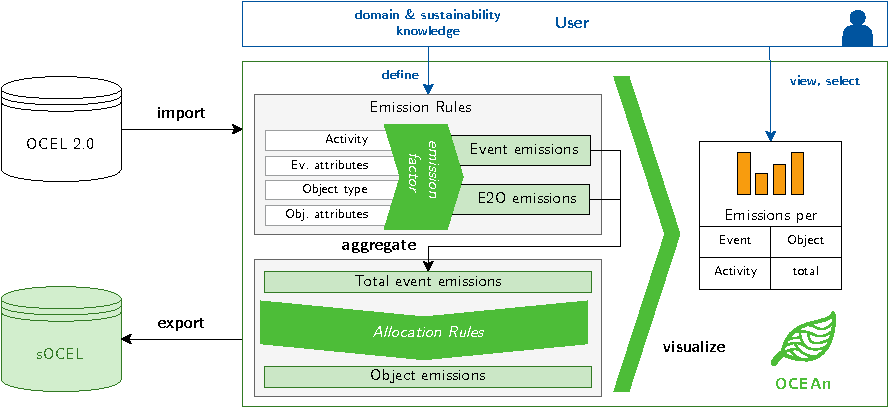
\includegraphics[width=.9\textwidth]{figures/concept/method-overview-4-method.pdf}
    \end{center}
    \caption{Schematic view of our method. After importing an OCEL, emission rules are defined by the user and applied to estimate emissions on event or event-to-object level (phase 1). Following this, emissions are aggregated for events, or for objects using the object allocation framework (phase 2). Results are visualized to the user, and integrated into the (s)OCEL when exporting.}
    % \caption{Workflow when using the OCEAn app. After importing an OCEL, emission rules are defined and applied to estimate event emissions. Different allocation rules can then be applied in order to map these emissions to objects. Event emissions are integrated into the (s)OCEL when exporting, object emissions are visualized and exported separately.}
    \label{fig:method-overview}
  \end{small}
\end{figure}

The overall goal of our work is to develop a tool enabling emission analysis leveraging data contained in an event log in the OCEL~2.0~\cite{OCEL2} standard.
\autoref{fig:method-overview} shows how the methods used to achieve this are employed by the OCEAn application.
After importing an OCEL, the procedure is split into two phases.

Phase 1 first determines emission data based on the OCEL. The data is obtained by applying emission rules, using a specified emission factor and data from the OCEL to compute emission values on event or event-to-object (E2O) level.
\autoref{sec:est} further elaborates on this emission estimation process.

Phase 2 further processes emissions specified on event or E2O level to provide different perspectives.
First, an event perspective is obtained by performing a simple aggregation. This provides insights like emission-driving activities.
Second, the \textit{object allocation} framework is proposed, mapping emissions on event and E2O level to objects.
At its core, the framework uses different \textit{allocation rules} that identify those objects related most directly with each event.
Details of the framework and the emission rules are given in \autoref{sec:alloc}.

The OCEAn application provides a frontend to control the import and export of OCELs as well as the execution of both phases. It also visualizes the results obtained from executing both phases. Further implementation details are given in \autoref{chap:impl}.
In the following, both parts of the method are addressed.

% ---------------------------------------------------------------------
% ---------------------------------------------------------------------
\section{Emission Estimation}
\label{sec:est}
In order to compute emissions on event or E2O level,
we propose \textit{emission rules} that extract different types of data from an OCEL, and apply a selected emission factor
to determine concrete emissions.

Emission factors are real numbers stating a conversion of a given quantity to \COtwo{} equivalents.
These quantities can be of various units, depending on the activity.
Examples include
\begin{itemize}[itemsep=-1.5ex]
  \item \unit{\kWh} -- electricity from grid,
  \item \unit{\liter} -- fuel combustion,
  \item \unit{\pkm} \textit{(passenger-kilometers)} -- bus transportation,
  \item \unit{\tkm} \textit{(tonne-kilometers)} -- freight.
\end{itemize}

In OCELs, events and objects can be annotated with attribute values.
Each attribute is associated with a specific activity or object type.
The same is adopted for emission rules,
leading to emissions only being computed for events of a given activity.
To compute emissions for multiple activities in the process, multiple emission rules are defined and their results combined.
Moreover, OCELs can contain both attributes with numerical and categorical values.
Here, we only refer to numerical attributes to be used in emission rules.

The units pkm and tkm mentioned above are commonly used for computing transport emissions~\cite{Shirizadeh24climate}.
As they are composed of two quantities by multiplication, emission rules also support multiplying values of different attributes.

\begin{figure}[t]
  \begin{small}
    \begin{center}
      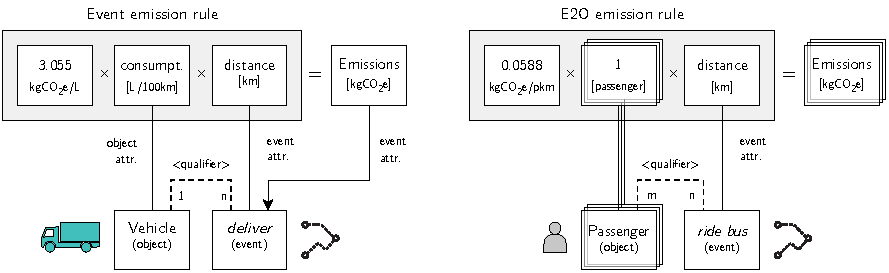
\includegraphics[width=\textwidth]{figures/concept/emission-rule-both-logistics-event-bus-e2o.pdf}
    \end{center}
    \caption{Emission rules using attributes of an event and associated objects. Left: Event emission rule, computing fuel-based emissions in a logistics process. Right: E2O emission rule, computing emission contribution per passenger in a bus transport.}
    % Emission factor sources: GEMIS, UBA\footnotemark}
    \label{fig:emission-rule-both-logistics-event-bus-e2o}
    % event - logistics:
    % ``Diesel - without biofuel content - used in vehicle''
    % https://www.climatiq.io/data/emission-factor/d56128ea-76e5-4a31-a6fe-b5e1ed855e52
    % Germany, GEMIS
    %
    % E2O - bus:
    % ``Emission intensity of diesel urban bus''
    % https://www.climatiq.io/data/emission-factor/06c42852-3f50-4f31-a86c-503d84b3eef5
    % Germany, UBA
  \end{small}
\end{figure}
% https://tex.stackexchange.com/questions/10181/using-footnote-in-a-figures-caption

In \autoref{sec:intro-motiv}, an example for computing emissions delivery events was given,
involving journey distance~[km] and average fuel consumption~[\unit{\liter\per\Ckm}], with example values:

\begin{align*}
	\qty{3.055}{\kgcotwoe\per\liter} \cdot \qty{12.5}{\liter\per\Ckm} \cdot \qty{20}{\km} &= \qty{7.6375}{\kgcotwoe}
  \;(\footnotemark)
\end{align*}
\nopagebreak
\footnotetext{
  \label{fn:factor-diesel-gemis}
  ``Emission intensity of diesel (without biofuel content) per liter used in vehicle''
  -- source: GEMIS
  (\url{https://www.climatiq.io/data/emission-factor/d56128ea-76e5-4a31-a6fe-b5e1ed855e52})
}
%
\autoref{fig:emission-rule-both-logistics-event-bus-e2o}~(left)
shows how this computation is represented by an emission rule:
Attribute values linked to the \otype{vehicle} object (consumption) and the \activity{deliver} event (distance) are multiplied with the emission factor, yielding an emission value for the event.
The result is later integrated into the OCEL as a new event attribute on the \activity{deliver} event.
This is part of the emission allocation framework introduced in \autoref{sec:alloc}.

In this example, emissions are computed on event level.
Still, a vehicle's object attribute value is used.
The value is well-defined because exactly one vehicle participates in the \activity{deliver} event.
Note that attributes of other objects from the logistics process (\autoref{tab:rex-ocel}), such as pallets, cannot be used this way:
The event \ev{deliver}{p2p3} is linked to multiple pallets (\texttt{p2} and \texttt{p3}), making \otype{pallet} a \textit{non-unique type} of the activity \activity{delivery}.

\begin{table}
  \caption{OCEL data usable in emission rules, depending on the level on which emissions are computed. Constant values, attributes of events and those object types uniquely associated with the activity are usable on both levels. E2O rules can additionally include attributes of the object type it is associated with. For the logistics example, the unique types per activity are listed on the right.}
  \label{tab:emission-rules-dtypes}
  \small
  \centering
  \begin{minipage}[t]{.575\textwidth}
    \strut\vspace*{-\baselineskip}\newline
    \begin{tabular}{r@{\ }lcc}
      \toprule
      \textbf{Data type} & & \multicolumn{2}{c}{\textbf{Usable in \dots}} \\
      && \makecell{Event \\ em. rule} & \makecell{E2O \\ em. rule} \\
      \midrule
      Constant && \faCheck & \faCheck \\
      Event attr. && \faCheck & \faCheck \\
      Object attr. & (of E2O object) & {\color{gray}\faTimes} & \faCheck \\
      Object attr. & (of unique type) & \faCheck & \faCheck \\
      Object attr. & (others) & {\color{gray}\faTimes} & {\color{gray}\faTimes} \\
      \bottomrule
    \end{tabular}
  \end{minipage}
  \hfill
  \begin{minipage}[t]{.375\textwidth}
    \strut\vspace*{-\baselineskip}\newline
    \begin{tabular}{rcccc}
      \toprule
      \textbf{Activity} & \multicolumn{4}{c}{\textbf{Unique types}} \\
      & {\color{order} \small\faFileInvoice}
      & {\color{item} \small\faList}
      & {\color{pallet} \small\faBox}
      & {\color{vehicle} \small\faTruck} \\
      & \hspace*{-.5em}{\color{order} \scriptsize ord}\hspace*{-.5em}
      & \hspace*{-.5em}{\color{item} \scriptsize item}\hspace*{-.5em}
      & \hspace*{-.5em}{\color{pallet} \scriptsize pllt}\hspace*{-.5em}
      & \hspace*{-.5em}{\color{vehicle} \scriptsize vhcl}\hspace*{-.5em} \\
      \midrule
      \activity{receive order} & \faCheck &  &  &  \\
      \activity{get item} & \faCheck & \faCheck &  &  \\
      \activity{load} & & {\color{gray}\faTimes} & \faCheck & \faCheck \\
      \activity{deliver} &  &  & {\color{gray}\faTimes} & \faCheck \\
      \activity{inspect} &  &  &  & \faCheck \\
      \bottomrule
    \end{tabular}
  \end{minipage}
\end{table}

In object-centric Petri nets, a process model introduced in OCPM,
this concept is represented by \textit{variable arcs}~\cite{vanderAalst20OCPNs}.
When an object type is not unique for a given activity, the arc between that activity's transition and a place associated with the object type is shown as a double arrow when visualizing the model.
For the logistics OCEL, the different activities' unique and non-unique object types are shown on the right side of \autoref{tab:emission-rules-dtypes}.
Object attributes of non-unique types can only be used by the second type of emission rules, \textit{E2O emission rules}, as shown on the left side of the table.

% , computing emissions on event-to-object (E2O) relation level.
% Here, each emission is linked to an event and an object. This allows 
E2O emission rules compute emissions on the level of E2O relations, with each result linked to an event and an object.
Therefore, the rule is defined for a specific activity and object type.
\autoref{fig:emission-rule-both-logistics-event-bus-e2o}~(right)
depicts such an allocation rule.
The example is from a different process, where multiple \otype{passengers} (represented as objects) are transported by a bus.
To employ an emission factor of the unit \unit{\kgcotwoe\per\pkm}, the passengers are usually counted. E2O emission rules work differently: A count of 1 is used in order to compute individual emission shares per \textit{passenger} object.
Thus, E2O emissions are obtained by
\begin{align*}
	\qty{0.0588}{\kgcotwoe\per\pkm} \cdot \qty{1}{\passenger} \cdot \qty{20}{\km} &= \qty{1.176}{\kgcotwoe}
  \;(\footnotemark).
\end{align*}
\nopagebreak
\footnotetext{
  \label{fn:factor-bus-uba}
  ``Emission intensity of diesel urban bus''
  -- source: UBA
  (\url{https://www.climatiq.io/data/emission-factor/06c42852-3f50-4f31-a86c-503d84b3eef5})
}

% with the emission result corresponding to one individual passenger.
The same computation is carried out for each passenger linked to the \activity{ride bus} event.
In the following step, these values are aggregated in order to obtain total event emissions.
This forms one part of \textit{emission allocation}, presented in the following section.

% ---------------------------------------------------------------------
% ---------------------------------------------------------------------

% ---------------------------------------------------------------------
% ---------------------------------------------------------------------
\section{Emission Allocation}
\label{sec:alloc}
The previous section showed how emissions can be determined using an OCEL.
In this section, these emissions are used to determine the total emissions associated with an event or an object.
To this end, the emissions are
\begin{enumerate}
  \item aggregated on event level in order to gain event and activity-based emission insights,
  \item allocated to a set of target objects, accumulating object carbon footprints.
\end{enumerate}

The input to both tasks consists of event emissions and event-to-object (E2O) emissions, both possible outcomes of applying emission rules as previously defined.
Note that all emission values are denoted as real numbers. We assume all of these quantities to be specified in kilograms of \COtwo{} equivalents (\unit{\kgcotwoe}).

To solve the first task, aggregation on event level is directly performed on the input data.
% The aggregated quantity $\emTot$ can be further used in order to compare event-level emissions and identify certain activites as emission drivers (\RGthree).

\begin{definition}[Total Event Emissions]
  Let $L$ be an OCEL, 
  $\emE\colon E\to\reals$ a function specifying every event's emissions,
  and $\emEtoO\colon E {\times} O \to \reals$ a function determining the event-to-object emissions where for all $e \in E$, $o \in O$: $o \not\in \objL(e) \implies \emEtoO(e, o) = 0$.
  % and the function $\emEtoO\colon E {\times} O \to \reals$ determining the object-specific event emissions where for all $e \in E$, $o \in O$: $o \not\in e2o(e) \implies \emEtoO(e, o) = 0$.
  For any $e \in E$ the total event emissions are denoted by
  $\emTot(e) \coloneqq \emE(e) + \sum_{o \in O} \emEtoO(e, o)$.
  \label{def:alloc-input}
\end{definition}

Computing $\emTot$ enables emission comparison on event level. The results can be further summarized by the event's activities. This allows identifying different activities from the process as emission drivers,
and is visualized in the OCEAn application using a bar plot.
%
For the second task, object allocation, a more sophisticated framework is proposed.

% ---------------------------------------------------------------------
% ---------------------------------------------------------------------
\subsection{Object Allocation Framework}
\label{sec:alloc-framework}
% ---------------------------------------------------------------------
% ---------------------------------------------------------------------

In order to perform LCA, emissions have to be aggregated along a product's lifecycle. This is enabled by the object allocation framework: Given emission data on event and E2O level, they are allocated to objects.

For this, we assume a given non-empty set of objects labeled as \textit{target objects} $\Omega\subseteq O$.

When distributing the event emissions among these target objects, the overall emissions have to be preserved:
All emissions associated with the process captured in the event log should be assigned to some object, and no additional emissions should be introduced or counted multiple times.

\begin{definition}[Valid Object Emissions]
  Given an OCEL \ocel, a set of target objects $\Omega \subseteq O$ with $\Omega \neq \emptyset$ and $\emTot\colon E\to\reals$, an object emission function $\emO\colon\Omega\to\reals$ is \textit{valid} if and only if the following invariant holds:
  \begin{equation*}
    \sum_{o \in \Omega} \emO(o) = \sum_{e \in E} \emTot(e)
  \end{equation*}
  \label{def:valid-obj-emissions}
\end{definition}

% Following this ensures the overall process emissions are fully distributed among the target objects.
Object emissions are composed of two intermediate components:

\begin{itemize}
  \item Target E2O emissions: E2O emissions that are directly associated with a target object.
  \item Allocated object emissions: emissions distributed among one or more objects via an allocation rule.
\end{itemize}

The second is directly obtained from input E2O emissions.

\begin{definition}[Target E2O Emissions]
  Let \ocel{} be an OCEL,  $\Omega \subseteq O$ a set of target objects with $\Omega \neq \emptyset$ and $\emEtoO\colon E {\times} O\to\reals$ the E2O emissions over \ocel.
  For $o \in O$ and $e\in E$, the \textit{target E2O emissions of $o$ in $e$} are given by
  \begin{equation*}
    \emEtoOmega(e, o) \coloneqq \begin{cases}
      \emEtoO(e, o) & \text{if } o \in \Omega \\
      0 & \text{else}.
    \end{cases}
  \end{equation*}
\end{definition}

Target E2O emissions form the only possibility how input emissions of the framework are directly connected to a single target object.
All remaining emissions are distributed to a set of target objects determined by applying an \textit{allocation rule}. Here, event emissions and (non-target) E2O emissions are no longer distinguished.
We denote the remaining event emissions of an event $e \in E$ by $\emRem(e) = \emE(e) + \sum_{o \in O\setminus \Omega} \emEtoO(e, o)$.

\begin{definition}[Allocated Object Emissions]
  Given an OCEL \ocel,
  a set of target objects $\Omega \subseteq O$ with $\Omega \neq \emptyset$,
  the remaining event emissions $\emRem(e)\colon E \to \reals$,
  and an allocation rule $\alpha\colon\allocruledef$, 
  % we define the allocated object emissions for all $o \in \Omega$, $e \in E$:
  for $o \in O$ and $e\in E$, the \textit{allocated object emissions of $o$ in $e$} are given by
  \begin{equation*}
    \emAlloc{\alpha}(e, o) \coloneqq \begin{cases}
      \frac{\emRem(e)}{\abs{\alpha(e)}} & \text{if } o \in \alpha(e) \\
      0 & \text{else}.
    \end{cases}
  \end{equation*}
\end{definition}

% Given $\emEtoOmega$ and $\emAlloc{\alpha}$,
An object's total emissions are determined by combining
its target E2O emissions and the emissions allocated to it by applying the allocation rule $\alpha$.
% In the following, both are combined in order to obtain the final result:

\begin{definition}[Object Emissions]
  Given an OCEL \ocel,
  a set of target objects $\Omega \subseteq O$ with $\Omega \neq \emptyset$,
  and an allocation rule $\alpha\colon\allocruledef$,
  the target object emissions of $o\in\Omega$ are computed as
  \begin{equation*}
    \emO(o) \coloneqq \sum_{e\in E} \bigl( \emEtoOmega(e,o) + \emAlloc{\alpha}(e,o) \bigr)
  \end{equation*}
  \label{def:obj-emissions}
\end{definition}

It can easily be shown that this definition always yields valid object emissions:
% \begin{lemma}
%   Object emissions computed as in \cref{def:obj-emissions} are valid object emissions.
% \end{lemma}

\begin{proof}
  Let $L$ be an OCEL, $\Omega\subseteq O$, $\Omega\neq\emptyset$ a set of target objects, $\alpha\colon\allocruledef$ an allocation rule, $\emE$ the event emissions and $\emEtoO$ the E2O emissions.
  Then for any $e\in E$,
  \begin{align*}
    \sum_{o \in \Omega} \emAlloc{\alpha}(e,o)
    &= \abs{\alpha(e)} \cdot \tfrac{\emRem(e)}{\abs{\alpha(e)}}
    = \emRem(e),
  \end{align*}
  so
  \begingroup
  \allowdisplaybreaks
  \begin{align*}
    \sum_{o \in \Omega} \emO(o)
      &= \sum_{o \in \Omega} \sum_{e\in E} \bigl(
        \emEtoOmega(e,o) + \emAlloc{\alpha}(e,o)
      \bigr) \\
      &= \sum_{e\in E} \Bigl(
        \sum_{o \in \Omega} \emEtoOmega(e,o) +
        \sum_{o \in \Omega} \emAlloc{\alpha}(e,o)
      \Bigr) \\
      &= \sum_{e\in E} \Bigl(
        \sum_{o \in \Omega} \emEtoO(e,o) + \emRem(e)
      \Bigr) \\
      &= \sum_{e\in E} \Bigl(
        \sum_{o \in \Omega} \emEtoO(e,o) + \emE(e) + \sum_{o \in O\setminus \Omega} \emEtoO(e, o)
      \Bigr) \\
      &= \sum_{e\in E} \Bigl(
        \emE(e) + \sum_{o \in O} \emEtoO(e,o)
      \Bigr)
      = \sum_{e \in E} \emTot(e)
      \qedhere
  \end{align*}
  \endgroup
\end{proof}


% ---------------------------------------------------------------------
% ---------------------------------------------------------------------
\subsection{Allocation Rules}
\label{sec:alloc-rules}
% ---------------------------------------------------------------------
% ---------------------------------------------------------------------

The previous section introduced the procedure used to distribute emissions among objects. The set of objects a given event's emissions are assigned to is determined using an allocation rule $\alpha\colon\allocruledef$.

This section provides a selection of such allocation rules.
% each assigning a non-empty set of target objects to a given event.
To give examples, the rules are applied to some events of the logistics event log (\autoref{tab:rex-ocel}). Emission-driving activities are ignored, assuming each event causes emissions of \qty{1}{\kgcotwoe}, leading to $\emRem(e)=1$ for all events $e \in E$. This is assumed for simplicity and to better demonstrate the impact of structures contained in the OCEL.
Emissions are to be allocated to the set of \otype{items}, so
\begin{align*}
  \Omega &= \allitms.
\end{align*}

\subsubsection*{AllTargets}
The trivial allocation rule assigns each event's emissions to all target objects, distributing the overall emissions evenly among them.

\begin{definition}[\allocrule{AllTargets}]
  Given an OCEL $L$ and a set of target objects $\Omegadef$,
  the \allocrule{AllTargets} allocation rule is defined by
  \begin{align*}
    \alphaAT(e)
    &\coloneqq \Omega.
  \end{align*}
  \label{def:AT}
\end{definition}

In the example, this distributes all emissions evenly among all items, disregarding the set of objects an event is related to. For the first two events, this leads to
\begin{align*}
  \alphaAT(\ev{receive}{o1}) &= \Omega = \allitms &
  \emAlloc{\alphaAT}(\ev{receive}{o1},o) &= \tfrac{1}{4} \;\forall o\in\Omega \\
  \alphaAT(\ev{get}{i1}) &= \Omega = \allitms &
  \emAlloc{\alphaAT}(\ev{get}{i1},o) &= \tfrac{1}{4} \;\forall o\in\Omega
\end{align*}

\subsubsection*{ParticipatingTargets}
Another rather obvious way to allocate an event's emissions considers those target objects directly participating in the event, distributing the emissions among them.
% This rule considers events that are directly related to target objects and distributes the event's emissions among them.
In case no target object participates in the event (like \ev{inspect}{v2}), the emissions are distributed among all target objects, like in the \allocrule{AllTargets} rule.

\begin{definition}[\allocrule{ParticipatingTargets}]
  Given an OCEL $L$ and a set of target objects $\Omegadef$,
  the \allocrule{ParticipatingTargets} allocation rule is defined by
  \begin{align*}
    \alphaPT(e)
    &\coloneqq \begin{cases}
      \objL(e) \cap\Omega & \text{if } \objL(e) \cap\Omega \neq\emptyset \\
      \Omega & \text{else}.
    \end{cases}
  \end{align*}
  \label{def:PT}
\end{definition}

Using this, emissions from the logistics process are allocated to those items related to each event, or to all items when there are none (like in \ev{inspect}{v2}).
\begin{align*}
  \alphaPT(\ev{load}{p3}) &= \bigl\{ \itm{3}, \itm{4} \bigr\} &
  \emAlloc{\alphaPT}&(\ev{load}{p3},-) = \bigl( \itm{3}\mapsto\tfrac{1}{2}, \itm{4}\mapsto\tfrac{1}{2} \bigr)
  \\ %
  \alphaPT(\ev{get}{i4}) &= \bigl\{ \itm{4} \bigr\} &
  \emAlloc{\alphaPT}&(\ev{get}{i4},\itm{4}) = 1
  \\ %
  \alphaPT(\ev{inspect}{v2}) &= \Omega = \allitms &
  \emAlloc{\alphaPT}&(\ev{inspect}{v2},o) = \tfrac{1}{4} \;\forall o\in\Omega
\end{align*}

\subsubsection*{ClosestTargets}
The previous rule only considers direct E2O relations for allocation.
Any events without relation to a target object are allocated to the complete set of target objects, not leveraging any process information further.

The \allocrule{ClosestTargets} rule uses the object interaction graph to derive distances between pairs of objects. Event emissions are then allocated to those target objects that have a minimal distance to an object related to the event.

\begin{definition}[\allocrule{ClosestTargets}]
  Given an OCEL $L$ and a set of target objects $\Omegadef$,
  the \allocrule{ClosestTargets} allocation rule is defined by
  \begin{align*}
    \alphaCTall(e)
    &\coloneqq
      \argmin_{o \in\Omega} \min_{o'\in\objL(e)} \dist{\OGOmegaL}(o,o').
  \end{align*}
  \label{def:CT}
\end{definition}

The definition implies the following for any event $e$:
In case $e$ has participating objects reachable from a target object,
$\alphaCTall(e)$ yields the closest target objects. Otherwise, $d(o,o')=\infty$ for all $o\in\Omega$ and $o'\in\objL(e)$, leading to $\alphaCTall(e)=\Omega$.

% Here, $\argmin$ is assumed to return the set of objects that share the same minimum distance to an object $o'$ related to $e$. This expression is well-defined: When there is no path in the underlying graph from any object related to $e$ to a target object, all targets are at distance $\infty$, leading to $\alphaCTall(e)=\Omega$.

\begin{figure}[t]
  \begin{small}
    \begin{center}
      \tikzset{auto shift/.style={auto=right,
      to path={ let \p1=(\tikztostart),\p2=(\tikztotarget),
      \n1={atan2(\y2-\y1,\x2-\x1)},\n2={\n1+180}
      in ($(\tikztostart.{\n1})!1mm!270:(\tikztotarget.{\n2})$) -- 
      ($(\tikztotarget.{\n2})!1mm!90:(\tikztostart.{\n1})$) \tikztonodes}}}
      \begin{tikzpicture}[
        event/.style={rectangle,draw=gray!50!black,fill=gray!25,inner sep=.2cm,minimum size=.6cm},
        object/.style={circle,draw,inner sep=.25em,font=\ttfamily},
        target object/.style={object,double},
        order/.style={object},
        item/.style={target object},
        pallet/.style={object},
        vehicle/.style={object},
      ]
        \node[item] (i1) {i1};
        \node[item,right=1cm of i1] (i2) {i2};
        \node[item,right=2cm of i2] (i3) {i3};
        \node[item,right=1cm of i3] (i4) {i4};
        \coordinate (n_i1_i2) at ($(i1.north)!.5!(i2.north)$);
        \coordinate (n_i3_i4) at ($(i3.north)!.5!(i4.north)$);
        \node[order,above=.75cm of n_i1_i2] (o1) {o1};
        \node[order,above=.75cm of n_i3_i4] (o2) {o2};
        \node[pallet,below=.75cm of i1] (p1) {p1};
        \node[pallet,below=.75cm of i2] (p2) {p2};
        % \node[pallet] (p3) at ($(i3)!.5!(i4) + (0,1cm)$) {p\_3};
        \coordinate (s_i3_i4) at ($(i3.south)!.5!(i4.south)$);
        \node[pallet,below=.75cm of s_i3_i4] (p3) {p3};
        \node[vehicle,below=.75cm of p1] (v1) {v1};
        \coordinate (s_p2_p3) at ($(p2.south)!.5!(p3.south)$);
        \node[vehicle,below=.75cm of s_p2_p3] (v2) {v2};
        %
        \node[event, left=2cm of o1] (receive_o1) {\ev{receive}{o1}};
        \node[event, right=2.5cm of v2] (deliver_p3) {\ev{deliver}{p3}};
        %
        \draw[densely dashed,color=gray!50!black] (receive_o1) -- (o1);
        \draw[densely dashed,color=gray!50!black] (deliver_p3) -- (p3);
        \draw[densely dashed,color=gray!50!black] (deliver_p3) -- (v2);
        \draw[->,densely dashed,color=gray!50!black] (o1) edge[auto shift] (i1);
        \draw[->,densely dashed,color=gray!50!black] (o1) edge[auto shift] (i2);
        \draw[->,densely dashed,color=gray!50!black] (p3) edge[auto shift] (i3);
        \draw[->,densely dashed,color=gray!50!black] (p3) edge[auto shift] (i4);
        \draw[->,densely dashed,color=gray!50!black] (v2) edge[auto shift] (i2);
        %
        \draw
          (o1) edge (i1) (o1) edge (i2)
          (o2) edge (i3) (o2) edge (i4)
          (i1) edge (p1)
          (p1) edge (v1)
          (i2) edge (p2)
          (i3) edge (p3) (i4) edge (p3)
          (p2) edge (v2) (p3) edge (v2)
          (i2) edge (v2) (i3) edge[auto shift] (v2)
          (p2) edge (p3);
        \draw[bend left=40] (i4) edge (v2);
        \draw[bend right=60] (i1) edge (v1);
      \end{tikzpicture}
    \end{center}
    \caption{Object interaction graph $\OGOmegaL$ of the logistics event log. Two objects are connected when they share some event. There are no edges between \otype{item} objects as they are all target objects (double borders). Two events are included as squares and connected to their participating objects, with the paths used for allocation depicted by arrows.}
    \label{fig:rex-og}
  \end{small}
\end{figure}

By definition, the object interaction graph $\OGOmegaL$ is constructed by object interactions, i.e., pairs of objects that participate in some shared event. For the logistics process (\autoref{tab:rex-ocel}), this graph is shown in \autoref{fig:rex-og}.
As the objects \texttt{i2}, \texttt{p2} and \texttt{v2} are all related to the event \ev{load}{p2}, they have pairwise edges.
%
Items that get loaded onto the same pallet are not connected in the graph. This is due to the fact that an extra edge between two target objects does not reduce the distance between a non-target and a closest target object. As items are set as targets, this makes all of them unconnected even though \texttt{i3} and \texttt{i4} both participate in the event \ev{load}{p3}.

Some events, including \ev{receive}{o1} and \ev{deliver}{p3} are not directly related to any \otype{item}. They are included in \autoref{fig:rex-og} and connected to their participating objects. Their emissions are allocated as follows:

\begin{align*}
  \alphaCTall(\ev{receive}{o1}) &= \bigl\{ \itm{1},\itm{2} \bigr\} &
  \emAlloc{\alphaCTall}&(\ev{receive}{o1},-) = \bigl(
    \itm{1}\mapsto\tfrac{1}{2},
    \itm{2}\mapsto\tfrac{1}{2}
  \bigr)
  \\ %
  \alphaCTall(\ev{deliver}{p3}) &= \bigl\{ \itm{2},\itm{3},\itm{4} \bigr\} &
  \emAlloc{\alphaCTall}&(\ev{deliver}{p3},-) = \bigl(
    \itm{2}\mapsto\tfrac{1}{3},
    \itm{3}\mapsto\tfrac{1}{3},
    \itm{4}\mapsto\tfrac{1}{3}
  \bigr)
\end{align*}

Compared to the previous rules, this allocation rule allocates more event emissions to proper subsets of the target objects. In fact, whenever $\alphaPT(e)\subsetneq\Omega$, \allocrule{ClosestTargets} returns the same result, because the participating target objects are at the minimal distance zero from themselves.
In \autoref{sec:alloc-props}, this is proven formally, along with other statements about allocation rule.

Still, \allocrule{ClosestTargets} allocates to large sets of target objects for some events, as seen in the example of \ev{deliver}{p3}:
As the \otype{item} \texttt{i2} is connected to the \otype{vehicle} \texttt{v2}, it receives emissions from a transport it is not involved in.
In the following, this issue is addressed by deriving a new object interaction graph based on a distinction between object types.

% ---------------------------------------------------------------------
% ---------------------------------------------------------------------
\subsection{Handling Units and Resources}
\label{sec:alloc-otcs}
% ---------------------------------------------------------------------
% ---------------------------------------------------------------------

In an OCEL, objects are the central elements connecting events with each other. As a contrast, in classical event logs, case IDs play a more well-defined role, representing instances of a process and at the same time a sequence of events.
While the lifecycle concept can be translated directly to an OCEL,
an object is not necessarily equivalent to a process instance. This gets clear when considering a few examples of certain object types in a process:
\begin{itemize}
  \item In the example logistics process (\autoref{tab:rex-ocel}), an \otype{order}, as well as an \otype{item} or \otype{pallet} is a suitable case notion. \otype{Vehicles} cannot be considered process instances, as their traces will grow large in a real-world dataset.
  \item In a sales process, a quotation or invoice can be considered a process instance. Products can be included as objects and linked to different quotations even when not translating to tangible objects. Assuming a product is offered permanently, its traces will contain events related to many different instances of that product.
  \item In a P2P process, an employee can be represented as an object and be related to different kinds of events they execute. However, an employee can handle multiple purchase requisitions at a time. Also, throughout their time at the company, they will handle a lot of purchase requisitions that might not be related at all.
\end{itemize}
Based on the above examples, we distinguish between
\begin{itemize}
  \item \textit{Handling units (HUs)}: Objects that can be considered \textit{cases} in the underlying process. A handling unit mostly has a limited lifetime within the process boundary, and may be an input or an output of the process. When two objects interact with the same handling unit in two different events, they are considered related to each other.
  
  Common examples of HUs are orders, invoices, packages, and documents.

  \item \textit{Resources}: Objects that can \textbf{not} be considered \textit{cases} in the underlying process. A resource mostly has a long lifetime or even exist throughout all the event log's timespan. Two objects interacting with the same resource are not considered to be related with each other.
  
  Common examples of resources are machines, employees, departments, and vehicles.
\end{itemize}

The object's role in the process provides another distinction: A process works \textit{on} HUs and \textit{with} resources.
Again considering the logistics example, \otype{orders}, \otype{items} and \otype{pallets} should be considered HUs, while a \otype{vehicle} is a resource as it is worked \textit{with}. This distinction can be made under the assumption that the number of events linked to a vehicle will be high in a larger dataset: The number of vehicles is constant, while each vehicle makes a number of rides each day over a long period of time.
%
As \otype{item} is an HU, two \otype{pallets} containing \otype{items} of the same \otype{order} are considered related, while two \otype{pallets} just loaded into the same \otype{vehicle} are not.

There is no exact definition in form of a quantitative requirement an object type has to satisfy to distinguish between HUs and resources.
In the following, this is assumed user input and denoted as
$\ObjHU$ and $\ObjResource$, two sets forming a partition of the set of objects.

% ---------------------------------------------------------------------
% ---------------------------------------------------------------------
\subsection{Object Interaction Graph Modifications}
\label{sec:alloc-og}
% ---------------------------------------------------------------------
% ---------------------------------------------------------------------

\autoref{sec:alloc-rules} introduced the \allocrule{ClosestTargets} rule that is using the object interaction graph $\OGOmegaL$.
This graph contains all objects of the event log as vertices,
and every two objects that share some common event or an O2O relation are connected by an edge.

As resources have long lifecycles with many events, they also interact with many other objects, leading to a high degree in the object interaction graph.
Also, by definition, two objects interacting with the same resource are not considered related with each other. Therefore, a shortest path used for allocation should not contain a resource, unless it is a target object itself.

When using the graph for allocating emissions from the logistics event log (\autoref{tab:rex-ocel}) to the \otype{items},
all items ever loaded to a \otype{vehicle} are at distance 1 from that vehicle. If an event of that vehicle is not directly related to any item, all those items at distance 1 will be assigned the event's emissions.
Here, the differentiation between HUs and resources comes into play. \otype{Vehicles} are resources and \otype{orders}, \otype{items} and \otype{pallets} are HUs. Interactions of \otype{items} and \otype{pallets} should be prioritized over those involving a \otype{vehicle}.
This is why another object interaction graph is proposed, just containing HUs.

\begin{definition}[HU Interaction Graph]
  For an OCEL $L$ with HUs $\ObjHU\subseteq O$ and a set of target objects $\Omega\subseteq O$ with $\Omega\neq\emptyset$,
  the \textit{HU interaction graph} is the undirected graph $\OGHUOmegaL$ with
  % \begin{align*}
  %   \OGHU(L) &= \restr{\OG(L)}{\ObjHU\cup\Omega}.
  % \end{align*}
  \begin{align*}
    % \Vertices\bigl(\OGHUOmegaL\bigr) &= \ObjHU\cup\Omega, \\
    \Vertices\bigl(\OGHUOmegaL\bigr) &= O, \\
    \Edges\bigl(\OGHUOmegaL\bigr) &=
      \Edges\bigl(\OGOmegaL\bigr) \,\cap\, \Pot\bigl( \ObjHU\cup\Omega \bigr).
  \end{align*}
  The \allocrule{ClosestTargets} allocation based on distances in $\OGHUOmegaL$ is denoted by $\alphaCTHU$.
  \label{def:og-hu}
\end{definition}

\begin{figure}[t]
  \begin{small}
    \begin{center}
      \tikzset{auto shift/.style={auto=right,
      to path={ let \p1=(\tikztostart),\p2=(\tikztotarget),
      \n1={atan2(\y2-\y1,\x2-\x1)},\n2={\n1+180}
      in ($(\tikztostart.{\n1})!1mm!270:(\tikztotarget.{\n2})$) -- 
      ($(\tikztotarget.{\n2})!1mm!90:(\tikztostart.{\n1})$) \tikztonodes}}}
      \begin{tikzpicture}[
        event/.style={rectangle,draw=gray!50!black,fill=gray!25,inner sep=.2cm,minimum size=.6cm},
        object/.style={circle,draw,inner sep=.25em,font=\ttfamily},
        target object/.style={object,double},
        order/.style={object},
        item/.style={target object},
        pallet/.style={object},
        vehicle/.style={object},
      ]
        \node[item] (i1) {i1};
        \node[item,right=1cm of i1] (i2) {i2};
        \node[item,right=2cm of i2] (i3) {i3};
        \node[item,right=1cm of i3] (i4) {i4};
        \coordinate (n_i1_i2) at ($(i1.north)!.5!(i2.north)$);
        \coordinate (n_i3_i4) at ($(i3.north)!.5!(i4.north)$);
        \node[order,above=.75cm of n_i1_i2] (o1) {o1};
        \node[order,above=.75cm of n_i3_i4] (o2) {o2};
        \node[pallet,below=.75cm of i1] (p1) {p1};
        \node[pallet,below=.75cm of i2] (p2) {p2};
        % \node[pallet] (p3) at ($(i3)!.5!(i4) + (0,1cm)$) {p\_3};
        \coordinate (s_i3_i4) at ($(i3.south)!.5!(i4.south)$);
        \node[pallet,below=.75cm of s_i3_i4] (p3) {p3};
        \node[vehicle,below=.75cm of p1] (v1) {v1};
        \coordinate (s_p2_p3) at ($(p2.south)!.5!(p3.south)$);
        \node[vehicle,below=.75cm of s_p2_p3] (v2) {v2};
        %
        \node[event, left=2cm of v1] (inspect_v1) {\ev{inspect}{v1}};
        \node[event, right=2.5cm of v2] (deliver_p3) {\ev{deliver}{p3}};
        %
        \draw[densely dashed,color=gray!50!black] (inspect_v1) -- (v1);
        \draw[densely dashed,color=gray!50!black] (deliver_p3) -- (p3);
        \draw[densely dashed,color=gray!50!black] (deliver_p3) -- (v2);
        \draw[->,densely dashed,color=gray!50!black] (p3) edge[auto shift] (i3);
        \draw[->,densely dashed,color=gray!50!black] (p3) edge[auto shift] (i4);
        \draw[->,densely dashed,color=gray!50!black] (v1) -- ($(v1)!.75cm!(i1)$);
        \draw[->,densely dashed,color=gray!50!black] (v1) -- ($(v1)!.75cm!(i2)$);
        \draw[->,densely dashed,color=gray!50!black] (v1) -- ($(v1)!.75cm!(i3)$);
        \draw[->,densely dashed,color=gray!50!black] (v1) -- ($(v1)!.75cm!(i4)$);
        % \draw[->,densely dashed,color=gray!50!black] (v2) edge[auto shift] (i2);
        %
        \draw
          (o1) edge (i1) (o1) edge (i2)
          (o2) edge (i3) (o2) edge (i4)
          (i1) edge (p1)
          % (p1) edge (v1)
          (i2) edge (p2)
          (i3) edge (p3) (i4) edge (p3)
          % (p2) edge (v2) (p3) edge (v2)
          % (i2) edge (v2) (i3) edge (v2)
          (p2) edge (p3);
        % \draw[bend left=40] (i4) edge (v2);
        % \draw[bend right=60] (i1) edge (v1);
      \end{tikzpicture}
    \end{center}
    \caption{HU interaction graph $\OGHUOmegaL$ of the logistics event log. \otype{Vehicles} do not have any edges as they are labeled as resources. Allocation paths for two events are highlighted, with \ev{inspect}{v1} now allocated to all four target objects.}
    \label{fig:rex-og-hu}
  \end{small}
\end{figure}

\autoref{fig:rex-og-hu} shows the HU interaction graph of the logistics event log. \otype{Vehicles} are considered resources, therefore they do not have any neighboring vertices. The edge set is reduced to interactions between HUs (orders, items and pallets). Again, there are no edges between \otype{items} according to \cref{def:og}, as they are all labeled target objects.

As \texttt{p3} is the only HU the event \ev{deliver}{p3} is related to, its emissions are allocated differently, this time not including the item \itm{2} that belongs to the other order.
\ev{inspect}{v1} relates to no HUs at all, so its emissions are distributed among all \otype{items}:

\begin{align*}
  \alphaCTHU(\ev{deliver}{p3}) &= \bigl\{ \itm{3},\itm{4} \bigr\} &
  \emAlloc{\alphaCTHU}&(\ev{deliver}{p3},-) = \bigl(
    \itm{3}\mapsto\tfrac{1}{2},
    \itm{4}\mapsto\tfrac{1}{2}
  \bigr)
  \\ %
  \alphaCTHU(\ev{inspect}{v1}) &= \allitms &
  \emAlloc{\alphaCTHU}&(\ev{inspect}{v1},o) = \tfrac{1}{4} \;\forall o\in\Omega
\end{align*}

In the previous example, the \otype{items} are labeled target objects. Therefore, they are mutually unconnected in both graphs (see \cref{def:og}).
Edges between objects of the same type are only present in \otype{pallets} that are delivered together.
In general, the non-target objects participating in the same event always form a clique in $\OGOmegaL$. In events with many objects, this leads to a high number of edges.

To reduce the edge number, another version of the object interaction graph is introduced, where edges between objects of the same type are always removed, regardless of whether they are target objects or not.

\begin{definition}[Object Interaction Graphs without Object Type Self-Loops]
  For an OCEL $L$ with HUs $\ObjHU\subseteq O$ and a set of target objects $\Omega\subseteq O$ with $\Omega\neq\emptyset$,
  the \textit{object interaction graph without object type self-loops} is the undirected graph
  $\OGxOmegaL$ with
  \begin{align*}
    \Vertices\bigl(\OGxOmegaL\bigr) &= O, \\
    \Edges\bigl(\OGxOmegaL\bigr) &=
      \Edges\bigl(\OGOmegaL\bigr)
      \;\setminus\;
      \Bigl\{ \{o_1,o_2\} \subseteq O \Bigm| \objtype(o_1) = \objtype(o_2) \Bigr\}.
  \end{align*}

  Analogously, the \textit{HU interaction graph without object type self-loops} is the undirected graph
  $\OGHUxOmegaL$ with
  \begin{align*}
    % \Vertices\bigl(\OGHUxOmegaL\bigr) &= \Vertices\bigl(\OGHUOmegaL\bigr) = \ObjHU\cup\Omega, \\
    \Vertices\bigl(\OGHUxOmegaL\bigr) &= O, \\
    \Edges\bigl(\OGHUxOmegaL\bigr) &=
      \Edges\bigl(\OGHUOmegaL\bigr)
      \;\setminus\;
      \Bigl\{ \{o_1,o_2\} \subseteq O \Bigm| \objtype(o_1) = \objtype(o_2) \Bigr\}.
  \end{align*}
  The \allocrule{ClosestTargets} allocation rules based on distances in $\OGxOmegaL$ and $\OGHUxOmegaL$ are denoted by $\alphaCTall^{\times}$ and $\alphaCTHU^{\times}$, respectively.
  \label{def:og-wo-ot-loops}
\end{definition}

Using these graphs, the question arises whether allocation results are preserved after removing object type self-loops.
This is assessed in \autoref{chap:eva} using large-scale event logs.
Also, the number of edges removed and the runtime reduction in distance computation is analyzed.
% Assuming there are always objects of more than one type participating in each event, distances between interacting objects of the same type will increase from 1 to 2 in 

% ---------------------------------------------------------------------
% ---------------------------------------------------------------------
\subsection{Allocation Properties}
\label{sec:alloc-props}
% ---------------------------------------------------------------------
% ---------------------------------------------------------------------

In order to compare the results obtained from object allocation, appropriate measures are required.
These measures are later used for the evaluation of the object allocation framework (\autoref{chap:eva}).
In the following, we assume an OCEL $L$, a set of target objects $\Omegadef$, and an allocation rule $\alpha\colon\allocruledef$.

The intermediate result of object allocation is the set of target objects an event gets allocated to, $\alpha(e)\subseteq\Omega$. The framework then computes a target emission distribution, $\emO$.
The allocation measures only make use of $\alpha(e)$ to provide an isolated evaluation of the allocation rule itself, disregarding the input emissions.

Two extreme cases in object allocation are events that get allocated to all target objects, and those being allocated to exactly one target object. The allocation measures are built around the frequency of these two cases.

\begin{definition}[Uniform and Unique Allocation]
  For an OCEL $L$, $\Omegadef$, an allocation rule $\alpha\colon\allocruledef$ and $e\in E$, we write that
  \begin{itemize}
    \item $e$ is allocated \textit{uniformly} using $\alpha$ if $\alpha(e)=\Omega$,
    \item $e$ is allocated \textit{uniquely} using $\alpha$ if $\abs{\alpha(e)}=1$.
  \end{itemize}
  Based on this,
  \begin{align*}
    \funiformalpha &\coloneqq \tfrac{1}{\abs{E}} \cdot
      \abs{\bigl\{ e \in E \bigm| \alpha(e)=\Omega \bigr\}}, \\
    \funiquealpha &\coloneqq \tfrac{1}{\abs{E}} \cdot
      \abs{\bigl\{ e \in E \bigm| \abs{\alpha(e)}=1 \bigr\}}.
  \end{align*}
\end{definition}

Note that $\funiformalpha + \funiquealpha \leq 1$. Equality is not reached in general, as events may be allocated to more than one, but not all target objects.
In the following, different statements for the previously defined allocation rules are made using these measures.

\begin{corollary}
  \phantom{Wer das liest ist blöd <3}

  \nopagebreak
  \begin{enumerate}[label={(\alph*)}]
    \item \allocrule{AllTargets} only allocates uniformly, i.e., $\funiform(\alphaAT) = 1$.
    \label{coroll:unif-a-AT}
    %
    \item \allocrule{ParticipatingTargets} allocates an event $e\in E$ uniformly if $\objL(e)\cap\Omega=\emptyset$.
    \label{coroll:unif-b-PT}
    %
    \item If \allocrule{ClosestTargets} allocates an event uniformly, so does \allocrule{ParticipatingTargets}. As a consequence, $\funiform(\alphaPT) \geq \funiform(\alphaCT{\OG})$ for every object interaction graph $\OG$.
    \label{coroll:unif-c-CT-PT}
    %
    \item If \allocrule{ParticipatingTargets} does not allocate uniformly, \allocrule{ClosestTargets} allocates to the same target objects.
    \label{coroll:unif-d-PT-CT-eq}
  \end{enumerate}
  \label{coroll:unif}
\end{corollary}

\begin{proof}
  \ref{coroll:unif-a-AT} and \ref{coroll:unif-b-PT} follow directly from Definitions \ref{def:AT} and \ref{def:PT}.
  \begin{enumerate}[label={(\alph*)}]
    % \item[(i)-(ii)]
    \setcounter{enumi}{2}
    %
    \item Let $L$ be an OCEL, $\Omegadef$ a set of target objects, and $\OG$ an undirected graph with $\Vertices(\OG)=O$. Now let $e\in E$ s.t. \allocrule{ClosestTargets} allocates $e$ uniformly, i.e., $\alphaCT{\OG}(e)=\Omega$. Then by \cref{def:CT} there is some $d\in\N_0$ s.t. $d=\min_{o'\in\objL(e)} \dist{\OG}(o,o')$ for all $o\in\Omega$.

    If $d=0$, then $\Omega\subseteq\objL(e)$.
    Otherwise, $\Omega\cap\objL(e)=\emptyset$.
    In both cases, \cref{def:PT} gives $\alphaPT(e)=\Omega$, i.e., \allocrule{ParticipatingTargets} allocates $e$ uniformly. \hfill$\square$
    %
    \item Let $L$ be an OCEL, $\Omegadef$ a set of target objects, and $\OG$ an undirected graph with $\Vertices(\OG)=O$. Now let $e\in E$ s.t. \allocrule{ParticipatingTargets} does not allocate $e$ uniformly, i.e., $\alphaPT(e) \subsetneq\Omega$. Then $\alphaPT(e)=\objL(e)\cap\Omega\neq\emptyset$ from \cref{def:PT}.
    As $\dist{\OG}(o,o)=0$ for all $o\in\objL(e)\cap\Omega$ and $\dist{\OG}(o,o')\geq 1$ for all $o\in\Omega\setminus\objL(e)$, and $o'\in\objL(e)$, \cref{def:CT} yields
    \begin{align*}
      \alphaCT{\OG}(e) &= \objL(e)\cap\Omega = \alphaPT(e). \qedhere
    \end{align*}
  \end{enumerate}
\end{proof}

Uniform allocation signals that allocation is not able to narrow down the set of target objects for a given event.
In contrast to that, unique allocation is the most precise result of allocating an event.
\autoref{chap:discussion} elaborates on this interpretation further.


% ---------------------------------------------------------------------
% ---------------------------------------------------------------------
